% vim:tw=0
% vim:fdm=syntax
\documentclass[a4paper,12pt]{scrartcl}
\usepackage{mythesis}
%
\author{Sakari Cajanus}
\studentnumber{82036R}
\email{sakari.cajanus@aalto.fi}

\title{Exercise Round 2}{Och samma på English}
\place{Espoo}
\thesisdegree{S-114.1100 Computational Science}{Bachelor's Thesis}
%\instructor{FT Mari Myllymäki}{Ph.D. Mari Myllymäki}
%\supervisor{TkT Markus Turunen}{D.Sc. (Tech.) Markus Turunen}

\uni{Aalto-yliopisto}{Aalto University}
\school{sähkötekniikan korkeakoulu}{School of Electrical Engineering}
\degreeprogram{Bioinformaatioteknologia}{Bioinformation technology}
\department{Lääketieteellisen tekniikan ja laskennallisen tieteen laitos}{Department of Biomedical Engineering and Excellence in Computational Science}
\keywords{suomeksi}{englanniksi}

\hypersetup{%
    colorlinks=true, linktocpage=false, pdfstartpage=1, pdfstartview=FitV,%
    % uncomment the following line if you want to have black links (e.g., for printing)
    %colorlinks=false, linktocpage=false, pdfborder={0 0 0}, pdfstartpage=3, pdfstartview=FitV,% 
    breaklinks=true, pdfpagemode=UseNone, pageanchor=true, pdfpagemode=UseOutlines,%
    plainpages=false, bookmarksnumbered, bookmarksopen=true, bookmarksopenlevel=1,%
    hypertexnames=true, pdfhighlight=/O,%hyperfootnotes=true,%nesting=true,%frenchlinks,%
    urlcolor=blue, linkcolor=blue, citecolor=green, %pagecolor=RoyalBlue,%
    %urlcolor=Black, linkcolor=Black, citecolor=Black, %pagecolor=Black,%
    pdftitle={\thetitle},%the title
    pdfauthor={\theauthor},%your name
    pdfsubject={\thetitle},%
    pdfkeywords={\thekeywords},%
    pdfcreator={XeLaTeX},%
    pdfproducer={A happy XeLaTeX user}%
}

\begin{document}
%\pagenumbering{roman}
\maketitlepage
\clearpage
\pagenumbering{arabic}
\section{Plots and conclusions}
In exercise round 2 we studied polynomial interpolation. In problem 4, we tried to approximate the \emph{serpentine curve}
\begin{align*}
f(x)=\frac{x}{1/4+x^2}
\end{align*}
using 13 equidistant nodes and again using 13 \emph{Chebyshev nodes} which were calculated using
\begin{align*}
	x_i=\frac{1}{2}(a+b) + \frac{1}{2}(b-a)\cos \left[ \left(\frac{i}{n} \right)\pi\right] \qquad(0\le i\le n).
\end{align*}
The interval $[a,b]$ used in both cases was $[-2.02857, 2.02857]$. In figure \ref{fig:curves} is shown our function itself and the two approximations. As predicted, the approximation done using \emph{Chebyshev nodes} is much better near the ends of our interval.
\begin{figure}[h!]
  \centering
    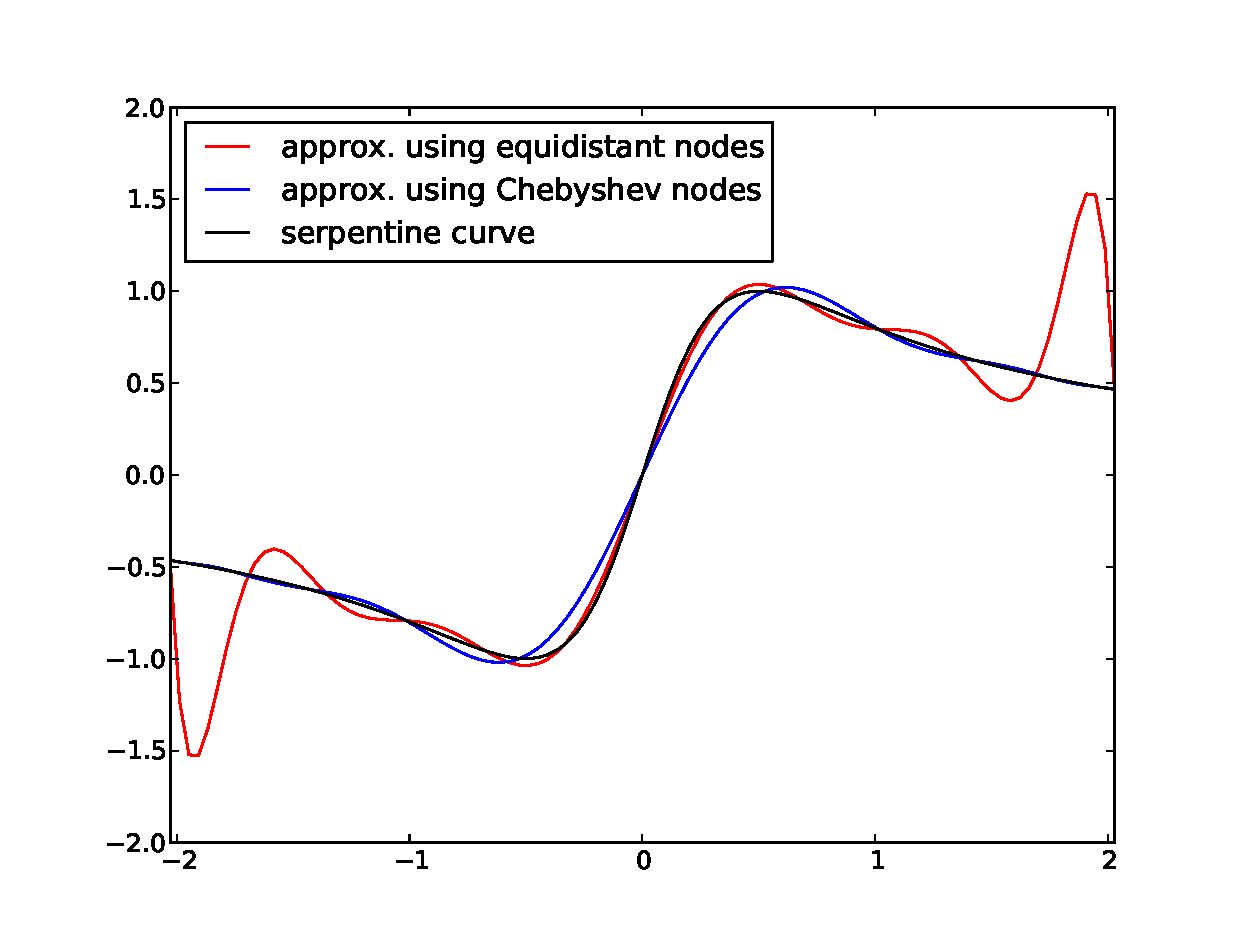
\includegraphics[width=0.7\textwidth]{curves}
  \caption{The serpentine curve and polynomial approximations}
  \label{fig:curves}
\end{figure}
However, as is shown in figure \ref{fig:errors} which shows us the errors $|p(x)-f(x)|$ calculated in 101 equidistant points in our interval, the error using \emph{Chebyshev nodes} is actually larger near zero. We can not be satisfied with the results, as better ways can be found to approximate this curve.

We usually choose to use \emph{Chebyshev nodes}, because they help to minimize the \emph{Runge's phenomenon}: problem of oscillation at the edges of an interval when using polynomials of high degree. In the case of \emph{serpentine curve}, approximation near the middle of the interval is also hard. 

As seen in figure \ref{fig:curves}, shape of the \emph{serpentine curve} is hard to approximate, even when using a polynomial of 12th degree. Better approximation might be possible if the points were chosen by hand. In this case, however, a good approximation could be done using natural cubic splines.
\begin{figure}[h!]
  \centering
    \includegraphics[width=0.7\textwidth]{errors}
  \caption{Errors of the polynomial approximations}
  \label{fig:errors}
\end{figure}
\clearpage
\appendix
\lstset{basicstyle=\ttfamily, numbers=left, numberstyle=\tiny, stepnumber=1, numbersep=5pt}
\gdef\thesection{Appendix \arabic{section}.}
\clearpage

\section{Code\label{LiiteA}}
\lstinputlisting[language=python]{ex2_pr4.py}
\end{document}
